% Created by Bonita Graham
% Last update: February 2019 By Kestutis Bendinskas

% Authors: 
% Please do not make changes to the preamble until after the solid line of %s.

\documentclass[10pt]{article}
\usepackage[explicit]{titlesec}
\setlength{\parindent}{0pt}
\setlength{\parskip}{1em}
\usepackage{hyphenat}
\usepackage[utf8]{inputenc}  
\usepackage{ragged2e}
\RaggedRight

% These commands change the font. If you do not have Garamond on your computer, you will need to install it.
\usepackage{garamondx}
\usepackage[T1]{fontenc}
\usepackage{amsmath, amsthm}
\usepackage{graphicx}
\usepackage{comment}

% This adjusts the underline to be in keeping with word processors.
\usepackage{soul}
\setul{.6pt}{.4pt}


% The following sets margins to 1 in. on top and bottom and .75 in on left and right, and remove page numbers.
\usepackage{geometry}
\geometry{vmargin={1in,1in}, hmargin={.75in, .75in}}
\usepackage{fancyhdr}
\pagestyle{fancy}
\fancyfoot[C]{\thepage}
\pagenumbering{gobble}
\renewcommand{\headrulewidth}{0.0pt}
\renewcommand{\footrulewidth}{0.0pt}

% These Commands create the label style for tables, figures and equations.
\usepackage[labelfont={footnotesize,bf} , textfont=footnotesize]{caption}
\captionsetup{labelformat=simple, labelsep=period}
\newcommand\num{\addtocounter{equation}{1}\tag{\theequation}}
\renewcommand{\theequation}{\arabic{equation}}
\makeatletter
\renewcommand\tagform@[1]{\maketag@@@ {\ignorespaces {\footnotesize{\textbf{Equation}}} #1.\unskip \@@italiccorr }}
\makeatother
\setlength{\intextsep}{10pt}
\setlength{\abovecaptionskip}{2pt}
\setlength{\belowcaptionskip}{-10pt}

\renewcommand{\textfraction}{0.10}
\renewcommand{\topfraction}{0.85}
\renewcommand{\bottomfraction}{0.85}
\renewcommand{\floatpagefraction}{0.90}

% These commands set the paragraph and line spacing
\titleformat{\section}
  {\normalfont}{\thesection}{1em}{\MakeUppercase{\textbf{#1}}}
\titlespacing\section{0pt}{0pt}{-10pt}
\titleformat{\subsection}
  {\normalfont}{\thesubsection}{1em}{\textit{#1}}
\titlespacing\subsection{0pt}{0pt}{-8pt}
\renewcommand{\baselinestretch}{1.15}

% This designs the title display style for the maketitle command
\makeatletter
\newcommand\sixteen{\@setfontsize\sixteen{16pt}{6}}
\renewcommand{\maketitle}{\bgroup\setlength{\parindent}{0pt}
\begin{flushleft}
\vspace{-.375in}
\sixteen\bfseries \@title
\medskip
\end{flushleft}
\textit{\@author}
\egroup}
\makeatother

\usepackage[backend=biber,bibencoding=utf8,style=ieee]{biblatex}
\addbibresource{references.bib}

% This styles the bibliography and citations.
%\usepackage[biblabel]{cite}
%\usepackage[sort&compress]{natbib}
%\setlength\bibindent{2em}
%\makeatletter
%\renewcommand\@biblabel[1]{\textbf{#1.}\hfill}
%\makeatother
%\renewcommand{\citenumfont}[1]{\textbf{#1}}
%\bibpunct{}{}{,~}{s}{,}{,}
%\setlength{\bibsep}{0pt plus 0.3ex}

%table package
\usepackage{booktabs}



%%%%%%%%%%%%%%%%%%%%%%%%%%%%%%%%%%%%%%%%%%%%%%%%%

% Authors: Add additional packages and new commands here.  
% Limit your use of new commands and special formatting.

\newcommand{\Gisli}{G\'isli Hj\'almt\'ysson}
\newcommand{\Steinar}{Steinar Sigurðsson}

% Place your title below. Use Title Capitalization.
%\title{SPOR - A lightweight consensus protocol for permitted blockchains}
%\title{SPOR - An elementary permitted block-chain}
%\title{A scaleable peer-to-peer consensus}
\title{Resource efficient peer-to-peer time-stamping service} 


% Add author information below. Communicating author is indicated by an asterisk, the affiliation is shown by superscripted lower case letter if several affiliations need to be noted.
\author{
\Gisli, \Steinar \\ \medskip \bigskip
Department of Computer Science, Reykjav\'ik University, Reykjav\'ik, Iceland  \\ 
%$^{b}$Department of CC, DD University, City, ST (italicized, state is listed as a two-capital letter designation)\\
\medskip \bigskip
https://www.ru.is/paper URL/ajur.2019.003\\ \medskip \bigskip
Student: steinars17@ru.is  \\
Mentor: gisli@ru.edu*
}

\thispagestyle{empty}
\begin{document}

% Makes the title and author information appear.
\vspace*{.01 in}
\maketitle
\vspace{.12 in}

% Abstracts are required.
\section*{abstract}
We believe that the primary value of any block-chain system is the creation of a totally ordered sequence of events in a distributed system, that is immutable and third party verifiable. We propose that all other functions, are in essence applications enabled from this basic functionality, and not seminal to function of the block-chain system. On the contrary, we argue that including functionality beyond what is essential to achieve this primary goal, introduces complexity beyond value, and is ultimately detrimental to the overall system performance and usefulness. In addition, and perhaps more importantly, we believe that distributed consensus protocols, whether academic such as Byzantine Generals Protocol and variations, or pragmatic as proof-of-work based consensus, do not take into account the different timescales of transaction processing on one hand, and that of node failures on the other, resulting in complexity, tight coupling, and lack of performance.

In this paper we propose a light-weight permitted block-chain system, having only the minimum functionality to ensure immutability, and third party verifiability. We show how this system provides high transaction rate while supporting a number of interesting applications.



% Keywords are required.
\section*{keywords} 
Blockchain; distributed consensus; immutable; high transaction rate

\vspace{.12 in}

% Start the main part of the manuscript here.
% Comment out section headings if inappropriate to your discipline.
% If you add additional section or subsection headings, use an asterisk * to avoid numbering. 

\newpage

\tableofcontents

\newpage

\pagenumbering{arabic}
\setcounter{page}{1}

\section{Introduction}
 
A confluence of changes is driving interest in block-chain related technologies, from consensus algorithms, to electronic money and asset management, to generalized smart contracts. The potential impact of block-chain technologies on areas such as trust management, open data exchange, and financial systems and services is substantial. The publication of \cite{satoshi-paper}, ushered in Bitcoin and cryptocurrencies as the primary driver of blockchain use. Since then a range of block-chain systems that have been proposed reflecting various trade-offs, commercial, academic , engineering, monetary and to some extent political/social \cite{satoshi-paper, hyperledger, byzantine, ethereum}. These systems, suffer from complexities to accommodate needs of unclear value, and lack of modularity due to intertwined mechanisms and policies. 

%Viewing these systems as distributed operating systems, ..., replacement of the worlds payment processing system, and even monetary system, has resulted in a variety of functionality beyond ... And lost focus on the principal functionally of the block chain system. 
\textbf{In particular, the two dominant block-chains \cite{satoshi-paper, ethereum} use proof-of-work (PoW) as their consensus mechanism,   }


In contrast we propose that the essential value of any block-chain system is the creation of a totally ordered sequence of events in a distributed system, that is immutable and third party verifiable. Furthermore, that all other functions of interest are in essence applications enabled by this basic functionality and not essential to the function of the block-chain system. On the contrary, we contend that including functionality beyond what is essential to provide these two seminal properties, reduces flexibility, introduces unwarranted complexity, and is ultimately detrimental to the overall system performance and usefulness.


We consider permissioned block-chains only, where a certain set of writers have the exclusive right to add to the chain. Additional members of the system can have read access to the system. Whereas, we don't put any upper limit on the size of the set of writers, the efficiency of our solution is negatively affected as this writer set grows without bounds. We are not aware of a situation where value is added by this set growing arbitrarily. 

Regardless of size of writer set, a more fundamental realization in our view is that we claim that such distributed system of substantial value will inherently be managed. Analyzing large scale networks demonstrates that networking systems are carefully designed, with valuable resources placed at strategic locations in the topology, with resources, redundancy and reliability reflecting the importance and value of such nodes \cite{Maltz2004}. 

The key observation is that even if only elementary measures are taken for the servers involved, failures of nodes occur at timescales several order of magnitude that of the timescale of transactions. Moreover, failures in a given round are not randomly distributed independent of previous rounds. The profound implication is that in all but pathological cases the cost of discovering the set of correctly working nodes is small. Persistently malfunctioning nodes (or even underperforming) may be removed by a slow-timescale writer group management protocol - potentially a human administrator. Of course the protocol must cope with failures occurring, but can be optimized for the common case.

Similar to other block-chains, we incorporate a mechanism for nodes to be rewarded for contributing to the construction of the chain, and consequently malfunctioning nodes to be penalized. However, rather than obfuscating the protocol with a new crypto-currency, by having the chain record the identity of the writer of each new block, the chain becomes a record of contribution suitable for any type of rewarding mechanism.

In this paper propose an elementary decentralized block-chain system built from only \textbf{three?} orthogonal mechanisms; i) a basic third-party verifiable event log, ii) a peer-to-peer consensus algorithm, and iii) %an external milestone certification. 
an active group management. 
We claim that a system having these seminal properties, is a powerful platform for a range of applications.

The contribution of this paper is a novel decentralized block-chain system, built from three elementary uncoupled components, that provides high transaction throughput, while supporting a range of applications of interest. We introduce a novel ultra light-weight consensus protocol, supporting very high transaction rate. Our analysis verifies the properties of the consensus protocol, complemented with simulation results to demonstrating the robustness and performance of the protocol. 

\emph{The rest of this paper is organized as follows. In Section 2 we discuss related work. In Section 3, we define the blockchain system and each of the three components of our lightweight system. Section 4, discusses implementation issues, analysis and discussion on the each of the three components, with Section 5 containing modeling and simulation. We then conclude in Section 6. } 


% We believe that these systems 
% Complexity
% Tight coupling of mechanisms and policies
% Lack of performance 
% Lack of flexibility

%decentralized, fair, lightweight, efficient and able to support high rate of transactions written to the blockchain.

% Aft4er decates of researching and operating networked and distributed systems we are not 
% aware # of any system operated by an organization for which these conditions would hold

% Reduced trust requirements
% Decentralized consensus
% Smart contracts 


%To play with:
%SPOR \\
%each event leaves an immutable imprint in history \\
%Orðstír  deyr aldrei \\
%ordstyrer (dansk) málamiðlari \\
%orðspor \\
%teikn \\
%traust \\
%Saga - saga systems, \\
%spor solutions \\
%Simple Pxxx Oxxx Record
%Elementary Event Imprint Record 

\section{Related work} 

In their 1999 paper, H. Massias et al \cite{massias} describe a "secure time-stamping service with minimal trust requirements", where a trusted third party issues timestamps upon client requests. Our basic immutable third-party verifiable event log is based on this work, albeit such that no single writer is trusted and is replaced by a peer-to-peer network of writers. 

Whereas \cite{massias, satoshi-paper} 
%\cite{possibly cite their HS91 and ?HS 97}
describe mechanisms to pack multiple client requests into a single block, any such mechanisms are orthogonal to our block-chain.

%\subsection{Byzantine agreement protocols}
%When dealing with asynchronous distributed systems, making sure each node in the system reaches an agreement on a single value is not trivial. Especially since any node can be faulty or malicious. 
The canonical problem of distributed consensus is the Byzantine generals problem.
Since this problem was introduced almost 40 years ago \cite{byzantine} a slew of papers have focused on various aspects and solutions \cite{bracha, PBFT}. The Byzantine generals problem has been shown to be tolerant to up to a third of the nodes being faulty or malicious.
%numerous protocols have been defined to make a system tolerant to these problems. These protocols are said to reach a Byzantine agreement, and the protocols can be tolerant for up to a third of the nodes in the system being faulty or malicious. In a modern permitted system it is unlikely that more than the third of the nodes become faulty which gives our system some margin to sacrifice tolerance for performance and throughput, and in the event that a big enough part of the nodes become faulty the event log will be reset to the last advertised state.

The Byzantine generals problem is formulated to reach a consensus \emph{one time} and hence the timescale of the single consensus is the same as the timescale of failures. 
The correctness criteria of a block-chain is weaker. The chain is a long log of events where blocks are only added to the chain if a consensus is reached. In our case a failure of even one writer prevents consensus of a given round. However, this does not impact correctness as the round is cancelled (see Section \ref{cancellation}), and merely reduces the overall performance in terms of transaction throughput. We show that under practical assumptions this impact is small.

%We only require that a consensus is observable and verifiable, when reached. In all other cases, the protocol may simply fail. As long as a sequence of consensus runs produces acceptable success rate, it is useful and valuable.
%Due to the separation of timescales the sequence of behaviors of writers and that the behavior is not independent between rounds and can be observed by a monitoring function. To ensure acceptable success rate, misbehaving nodes may be "voted off the island".

%General, bitcoin, etherium, xxx
Clearly, the most influential publication on block-chain is the "Satoshi" paper introducing Bitcoin \cite{satoshi-paper}. Similar to \cite{satoshi-paper} we base our immutable event log on \cite{massias}. However, rather than introducing PoW to select the winner of each round, we take a protocol approach, avoiding the resource consumption of Bitcoin hashing altogether. Whereas the effort and cost of hashing may potentially be justified for Bitcoin as the Bitcoin and its use is \emph{the} proposed value of the Bitcoin chain, the growing resource consumption seems unsustainable and to threaten the viability of the Bitcoin block-chain. In contrast, our resource-light protocol focuses on the value embedded in the body of each block, the immutability, and the total order logged by the chain.


%\subsection{Bitcoin} \cite{satoshi} \\
%It is unclear to the authors that air-conditioning shopping malls is somehow more noble use of electricity that to power up Bitcoin miners.The observed increasing value of Bitcoin, would seem justified it it reflected value perceived by the ledger, e.g. from increasing demand to write into the ledger. But it does not. The cost of Bitcoin is not driven by demand from clients wishing to have transactions written to the chain. On the contrary, the total value of the ledger and its content is not positively related to the value of Bitcoin or the total number of miners. Hence, from an engineering point of view, beyond a certain (relatively small) number of miners, doubling the number of miners mining for Bitcoin, doubles the cost of the system without increasing the value produced by the ledger. 


%\subsection{Ethereum}
The Bitcoin blockchain is created for one application only, namely digital cash\footnote{We acknowledge that users are using it for other applications including smart contracts.}. Ethereum \cite{ethereum} adds smart-contract functionality, whereby each transaction implements an arbitrary functionality, executed by the block-chain system. This introduces substantial complexity into Ethereum system and unpredictability in the execution of transactions. Adding to the chain is the \emph{critical section} of the underlying distributed system. It seems contrary to the learning of the operating systems and distributed systems community to introduce substantial complexity and unpredictability into the critical section. 

From the perspective of this research, smart contracts and their execution should be carried out separately from the underlying block-chain system. 

This view resonates with the approach taken by the IBM Hyperledger \cite{hyperledger}. IBM promotes the Hyperledger as a distributed operating system based on block-chain, with a very generic model for smart-contracts, supporting in principle smart-contracts based on any programming language. However, although the execution of smart contracts is the responsibility of the Hyperledger system, their execution is part of preparing a proposed transaction, before such transaction is submitted for addition to the block-chain, and therefore executed outside of the critical-section where the block is added.

Our approach takes one step further, pushing the management and execution of smart-contracts further out, and completely out of the block-chain system. We are aware of and involved in some exciting work on smart-contracts \textbf{CITE - what paper?}, and see substantial potential in such research. However, we propose that a smart-contract system be built on top of our lightweight block-chain, as an application.

Following the success of Bitcoin, many new cryptocurrencies have been launched, and the majority of them use the PoW consensus algorithm \cite{sadek2020blockchain}, in spite of its high energy consumption and poor scalability. To combat these limitation, a proof-of-stake (PoS) system has been introduced and used by some blockchains. PoS requires no puzzle to be solved and therefore circumvents the energy problem, but it is not as secure as PoW systems. They have more miners and have better decentralization than PoS, which gives a higher probability of collusion among validators. Our lightweight blockchain introduces a new consensus algorithm. It does not require high energy consumption and it is highly secure, as we will discuss in Section \ref{blockchain-system}

A similar solution to the consensus problem was proposed by Finlow-Bates \cite{finlow2017lightweight} in 2017. His solution consisted of giving each writer a specific identification number. When a new block is written, the chain is given some calculated score and the writer with the identification number closest to that score, gets to write the next block.
While this solution is lightweight and computationally inexpensive, it is susceptible to ``stake grinding'' \cite{onstake} attack from two or more colluding writers. When a writer wins a round and gets to write the next block to the chain, he could add some nonce value that would alter the new chain score such that it is closest to his colluding partner's identification number. 
In contrast, since our solution to the problem is in short to calculate the xor of a generated number from all participants, it is impossible to collude and predict the result from the calculated score, unless all participant are colluding together, in which the protocol would reach consensus.

The notion of implementing blockchains in the Internet of Things (IoT) has been divisive between developers. The combination of the two can be powerful as blockchains bring a lot of advantages to the table, especially their decentralization and immutability. Christidis et al.\cite{christidis2016blockchains} examined this combination thoroughly and stated the advantages and disatvantages of blockchains in IoT. One of the main problems they found was that blockchains have lower transaction processing throughput than a normal centralized database and higher latency, especially with the PoW blockchains. The lightweight consensus protocol we propose is efficient and has high throughput which is limited only by the network latency from the device.



\section{The blockchain system}

We define a blockchain system as a set of nodes with the common objective of writing and verifying a single totally ordered chain of transaction blocks. 

A subset of the nodes are \emph{writers} that are allowed to write new blocks to the chain. Writers participate in a (distributed) consensus algorithm to determine a winner, who gets to write the next block. The set of writers $W$ may change dynamically, although  the changes to the membership are assumed occur at timescales several orders of magnitude larger than that of transactions.  
Nodes that are not writers are  either clients, generating transaction requests, or observers, all of which can read the entire chain, and verify that the chain is validly construed. %In this paper we focus on the writers.
Writers communicate directly over the Internet, essentially forming a peer-to-peer network. Some messages may be lost in this peer-to-peer network. 

Nodes may be rewarded for writing to the block\footnote{Not necessarily with direct monetary reward, but could be any type of recognition} or otherwise desire to write to the block but may misbehave to gain an advantage, or attempt to rewrite part of the chain. Clearly, nodes can fail and may maliciously attempt to game the system, or simply prevent it from functioning.

In what has become referred to as public chains, including the Bitcoin block-chain, all nodes are potential writers and equal with respect to their privileges and participate equally in the consensus protocol.

%% one of the problems with this of course is lack of scalability and performance


\subsection{Generalized permitted chains}
We define a permitted chain to a be a block-chain system where the set of writers $W$ consists of nodes that are explicitly \emph{permitted} into the set of writers. The changes in the membership are thus governed by some additional protocol and policy. Whereas this introduces some complexity in terms of managing the membership of writers, we observe, that the time scale of such management is orders of magnitude that of the processing transactions. 
%, and thus believe that the value added by managing the membership will far outweigh the cost of complexity (this is clear from the Internet). 
For those permitted chains that we know of, this management is off-line. No assumptions are made about the number of writers or their distribution. A permitted chain only limits the priviledges of writers, but is publicly open to any client or observer. 

%[Below we discuss mechanisms and protocols to monitor, and dynamically adjust the set of writers, for example based on performance, fairness, and other policies.] Do we?

\section{The lightweight Blockchain system}
\label{blockchain-system}
In this section we describe the three main mechanisms of our blockchain system. First, an elementary event log built on a peer-to-peer time-stamping service. Second, we define and describe the lightweight decentralized consensus protocol. Third, the management and monitoring of the group of writers.


\subsection{A simple light-weight event log}

\begin{figure}
    \centering
    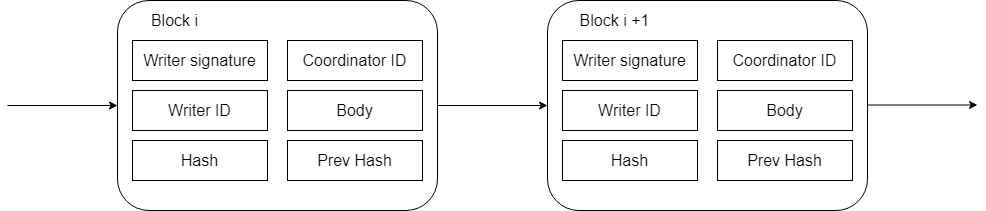
\includegraphics[scale=0.4]{images/chain.png}
    %\vspace{0.2}
    \caption{An immutable chain of events}
    \label{fig:my_label}
\end{figure}

Our event log is essentially a timestamp server, similar to that described in \cite{massias} and adopted for Bitcoin. Each entry in the log consists of, i) the id of the coordinator, ii) the id of the winner, iii) the body, iv) the hash of the block, v) the hash of the previous block, and vi) the signature of the writer of the block (i.e. the winner).
The critical element is that the hash of the block includes the hash of the previous entry in its hash. By induction the hash value of the new block is a function of all previous blocks, providing the immutability of the chain with respect to the set of writers. The body may be composed of multiple transactions that may be further organized e.g. into Merkle trees \cite{Mercle1980}.
Such optimizations are not the topic of this paper.

The chain is immutable as no previous block cannot be changed without the participation of \emph{ALL} members of the writer group. Each block is signed cryptographically by the winner who writes it. Moreover, any rewrite could be cancelled by any writer in the group. Most importantly, such rewriting would be clear and obviously detected by any of the writers. Thus, %contrary to claims in \cite{satoshi-paper}, 
\textbf{our time-stamping service is peer-to-peer without proof of work}. 


\subsubsection*{Milestoning and immutability}
To further make the event log immutable beyond the set of active writers, periodically a milestone event is added to the chain, and publicized widely. The first milestone event is the genesis block. For publication any persistent publicly accessible forum will do, for example a Usenet or a Facebook post. For our implementation, we add a milestone event for every 100K events, by writing the milestone event into the Bitcoin block-chain. 

Publicizing the event seals the immutability of the chain. Even if the chain is private and only accessible to a limited set of readers outside the writer group, for example external auditors, the public milestones serve as external anchors to the chain. Even if the chain exists for a limited time, and the set of writers is retired, the last milestone serves as the end of chain, which again cannot be altered thereafter without it being detectable.

\subsection{A lightweight high-performance consensus protocol}

For a high level view of the underlying idea of the lightweight decentralized 
consensus protocol, we select a leader based on the following. Each writer has a private
cryptographically secure one-time pad (OTP) \cite{Vernam1926}. In each round, each writer 
produces the next number from its  OTP. From all the numbers we calculate 
an aggregate result, i.e. a generalized "sum". The writer whose number is 
closest to the aggregate is declared the leader.

%More formally, we define a set $W$ set of writers. We wish to consider consensus protocol, that works an arbitrary size of the set of writers. 
%2 and infinity as limiting cases of $||W||$.

\subsubsection*{The consensus protocol}
To formalize the above idea into a protocol, we define a set $W$ set of writers, and  start by considering a single round. First we enumerate the set of writers, from 0 to $||W|| - 1$. For each round a \emph{coordinator} is selected (described below), to coordinate the round. The Coordinator does not participate in the round as a contender to win. All arithmetic
is performed modulus some large $N$. The round is in four steps:
\begin{itemize}
    \item Step 1: The Coordinator broadcasts to all other writers in $W$ a request for the next number.
    \item Step 2: Each writer, generates the next number from its local OTP, and responds by transmitting it to the Coordinator.
    \item Step 3: The Coordinator, aggregates the numbers into a result $r$, and determines the winner, $w$, as the identity of the writer whose number is "closest" to $r$. The Coordinator then broadcasts to all writers in $W$, the result $r$, the winner $w$, and all numbers received in Step 2.
    \item Step 4: Each writer, verifies the round by confirming i) that its number is correctly received and reported, ii) the calculation of $r$, and thus iii) the winner $w$. The winner broadcasts its winning block, cryptographically signed. All others, if all is correct, reply with a confirm to the coordinator. Otherwise, a dissenting writer \emph{broadcasts} a reject.
\end{itemize}

%\footnote{Question if we should cancel rounds for which less than 50\% participate}
%Sure, en það gerist mjög sjaldan, Gæti verið af öryggisástæðum

For the initial round the writer with the lowest number acts as the round coordinator. For subsequent rounds we have used a simple round robin. 
%Alternatively one could have the winner of round $i$ be the coordinator for round $i+1$. 

To aggregate the number from all the writers, we could in principle use a simple summation modulus $N$. For its simplicity when working with large numbers (e.g. multiple words) and for its cryptographic properties, we have chosen to use XOR as the aggregation function.

The distance metric is more tricky. We can think off, and have experimented with a number of distance metrics, including i) the arithmetic difference, ii) the Hamming distance, iii) the value of the result XOR-ed to each value, i.e. $r \oplus s_i$, where $s_i$ is the number generated by writer $w_i$. 

To break ties we have used the enumerated identity of $w$. Whereas, more elaborate tie breaking exist, with $N$ large enough, the likelihood of ties is small.

%NEED to resolve - Who writes the block, how is the block communicated to others. 
%How does this happen in Bitcoin and Etherium? [Steinar help]

%BITCOIN: p2p network where full nodes (nodes that have the entire bitcoin database downloaded) verify all blocks they receive before they relay the information to other nodes. Nodes can request a getBlock message to other synced nodes where they specify which block is their newest block, and synced block finds it's most trusted local chain, and sends back a number of blocks starting with the requesters block number + 1. The requester then verifies each block and adds it to its local chain. When a writer 'discovers' a block, he broadcasts that block to all connected nodes, who verify the block. Either sending an inv messages or just straight up send the block it self, skipping the inv - getblock stage.

%ETHEREUM: each new node is hardcoded to connect with 3 nodes, that are maintained by ethereum foundation (centralization in a decentralized system?) These nodes connect the new node to known ethereum nodes, and you are connected to the network. Ethereum uses TCP connections. Miners are separate nodes, they solve a puzzle (similar to bitcoin), winner gathers all transactions, put them into the block, and then write the block to their local chain and broadcast the block to the other miners on that ethereum chain.

\subsubsection*{Message complexity}

%Breyta til að taka tillit til new Step 4

The message complexity is $||W||-1$ messages of fixed size for each step one and two. For step three $||W||$ messages each of size $||W||$. For step four, if no writer dissents,  $||W||-2$ messages of fixed size are sent to the coordinator, 
plus $||W||-1$ messages from the winner to transmit the new block to all. 
Hence for successful rounds the number of messages becomes $o(||W||)$.

If the round fails, each dissenting writer broadcast a message, in which case the complexity becomes $c * ||W||$, where $c$ is the number of cancelling nodes.  To avoid this last broadcast, the protocol can be augmented by adding one extra round of messages, where the coordinator broadcasts a cancel if one is received. However, in the situations that we are targeting, we foresee that $c$ to be too small for this to affect the overall performance of the protocol. 

Another potential issue is the the size of the message in Step 3 is $||W||$. For the numbers we envision for the set of writers, e.g. no more than few hundreds, it is not an issue. For larger sets, without affecting the correctness of the protocol, the coordinator may omit sending the numbers received from all and simply announce the result by broadcasting the result and the identity of the winner.

To prevent any bias and reduce the dependency of the coordinator, the protocol could be elaborated by using two or more coordinators, which all play the role of the coordinator and do not participate in the protocol to be selected as potential winners. With multiple coordinators, any mismatch between coordinators would render such round cancelled.

Alternatively, a monitor may be nominated, either as a separate node, or as a rolling function among the writer set, allowing the monitoring of biases, collusion and other misbehavior, ruling out misbehaving nodes. For a number of reasons, including debugging, in our work we include such a monitor as a matter of course.

%All players establish a secure connection with the host. The host receives a number %from all players and then sends all numbers back to the players as well as the winner


\subsubsection*{Correctness}

The purpose of the consensus algorithm is in each round to select the writer $w$ that becomes the leader, i.e. gets to write to the chain. Each process draws from its OTP an initial value. The goal of the protocol is that all valid writers decide on a value $v$. The problem can be formally defined in terms of three properties:
\begin{itemize}
    \item Validity: If all correct writers propose the same value $w$, then any correct process that decides, decides $w$.
    \item Agreement: No two correct writers decide differently.
    \item Termination: Every correct process eventually decides.
\end{itemize}

The first two properties ensure correctness, whereas the last ensures termination \cite{Alpern-Schneider}. 

The value $w$ is broadcast in Step 3, and verified by each writer in Step 4. If the coordinator is faulty it may select a writer $\vec{v}$. In any case, if a writer does not concur with the result, regardless of the reason, then such a writer will trigger a cancel. Hence, if no cancel occurs, all processes in the writer set (including the coordinator) will decide on the same value $w$, thus establishing correctness. Clearly, every correct process will eventually respond, and thus decide.



\subsubsection*{Performance enhancements}
%Overlapping of rounds}
It is clear that the latency (from beginning to end) of the protocol is two round-trips. However to enhance the throughput, it is worth observing that the next round does not need to await the completion of the previous round. Rather, the next coordinator in line, having generated its response and completed Step 2, of round $i$, immediately initiates round $i+1$, and so on. The result is that the latency from beginning of one round to the beginning of the next is the \emph{one way} latency in the network of writers.

%\subsubsection{Batching}
To increase the transaction rate further, one can adopt a similar approach to for example the Bitcoin block-chain, where multiple transactions are written in each block, effectively scaling the transaction rate by a constant. Alternatively, in each round, rather than generating a single number, each writer can generate $k$ next numbers from the OTP, resulting in $k$ next winners being selected in each round.




\subsection{Managing the set of writers +}
%% Typically $W$ is established by a God-node or off-line by configuration

We consider the membership and management of the groups of writers. 

To create a new lightweight block-chain, a creator prepares a configuration containing a list of permitted participants and distributes it to the participants as a way of invitation. One easy way to do this is to simply publish the list at a forum known and accessible to the participants, e.g. on the web. Each participant retrieves the list of invitees, verifies their identities and public keys, and joins the peer-to-peer network of writers by initiating a session with one or more of the participants. Participants may be designated as writers, readers, clients or monitors. The configuration may include additional properties, such as number of coordinators per round and more. The block-chain may be open to readers and/or clients. In that case anyone will be admitted for read access, and/or as a new client issuing requests.

Each writer maintains a state for every writer in the writing set. This state includes, the writers id, and public key, but also the protocol state of the writer, either active or penalty. In addition writers may keep track of statistics of other writers and more.

The basic protocol deals with occasional message losses as message losses will either result in timeout and subsequent retransmission, or will simply trigger a cancel. For smaller writer sets, we have implemented the peer-to-peer networks as a fully connected mesh, with reliable delivery (TCP). 

Connectivity of the peer-to-peer network connecting the group of writers is maintained separately from the consensus protocol and block-chain management. Using a relatively simple echo-reply style protocol, disconnected nodes can be %relatively easily
identified. At the protocol level, such nodes are treated as being in the penalty box.


%%	Can determine membership changes in writer set relatively fast
%%	Thus can assume - size of connected nodes is stable \\
%%Node not responding in three clock ticks is deemed dead
%	Only an issue if majority of nodes do not respond
%Issue: what if node owning "MUTEX" i.e. the right to write, i.e. the leader dies.
%	Resolution?: majority of prior leaders override 
%	Not robust to the winner misbehaving after being elected


%\subsubsection*{Must deal with +}
%Malicious leader
%Faulty leaders
%partitions






\section{Failures and cancelled rounds}
\label{cancellation}
A round fails if any of the writers fails to confirm the consensus (in step 4). This occurs if for some reason the verification step fails, if for any reason a writer fails to respond (time-out), or otherwise fails. Our failure model and operating assumption make writer failures unlikely, however when a writer fails, it will be in a failed state for a number of rounds. To reduce the impact of failures on the overall throughput of the system, a failed writer is put into a penalty box (i.e. a suspend list) where it remains for some amount of time until it is allowed back as an active writer.


%\subsection{writer failure}

%The cancellation policy treats each cancelled round as a failure. 
When a player faults (whatever the reason), it enters the penalty box initially for four rounds. If the writer is still faulty, when the penalty expires, the penalty time is doubled, resulting in exponentially increasing penalty time, thereby limiting the number of rounds affected by a failure of a particular writer. For practical reasons, we implement a maximum penalty time.

%To combat this, we propose putting an upper limit on the backoff time at one hour. That keeps the number of cancelled rounds down and moves the worst case down to only 5 hours waited. This policy also discourages malicious players to cancel each round the don't win. If a player cancels a round to boost it's average number of won rounds, it will miss 4, then 8, then 16 and so on rounds, which puts them at a disadvantage.

%\subsection{the exponential backoff}
%Every writer manages a lookup table for each player, and when some writer broadcasts a cancelled round, the other writers add their backoff time to their lookup table. When a new round starts and the new coordinator of the round is chosen, the writers check (betra orð) the lookup table make sure that the writer is not in timeout.

%\subsection{coordinator failure}
If a coordinator is faulty, it will be observed by multiple writers, each of which broadcasts a cancel message. Thus the round is cancelled, and the protocol moves on.


\section{Analysis and Modeling}
In this section we analyze some of the properties of the protocol and model the throughput performance. We start with formalizing the following definition of the sequence of winners.


%\subsection{Lightweight decentralized consensus}
%Consider $Z_n$ the set of non-negative integers less than $n$. 
%Let $\vec{\sigma_i}$ be a sequence, $\sigma_{i,0}, \sigma_{i,1}, \sigma_{i,2}, ...$ such that 5$\sigma_{i,t}$ is in $Z_n$ for all $t \ge 0$, and where $\vec{\sigma_i}$ is the sequence %generated by writer $i$. We say that $\sigma_{i,t}$ is the number generated by node $i$ at %round $t$.


%The basic consensus protocol works as follows. For each round, $t$, each writer, transmits their respective $\sigma_{i,t}$ to the coordinator. The coordinator  
%having received the latest number from everyone else for round $t$ 	
%55\begin{itemize}
%    \item computes a sum $s_t$ in $Z_n$ of all the numbers received, i.e. $s_t = \sum s_{j,t} %\forall j$
%    \item Computes winner as min distance from $s_t$, i.e. \(
%		\{ k : || s_t - s_{k,t} || \leq || s_t - s_{j,t} || \hspace{4} \forall j \} \)
%|	\item Declares node $k$ as the winner of the round (in case of tie select the lowest %numbered $k$).
%\end{itemize}

%Node $k$, the winner, writes next entry to the log.



\subsection{A distributed one-time-pad}
Consider $Z_n$ the set of non-negative integers less than $n$. 
Let $\vec{\sigma_i}$ be a sequence, $\sigma_{i,0}, \sigma_{i,1}, \sigma_{i,2}, ...$ such that $\sigma_{i,t}$ is in $Z_n$ for all $t \ge 0$, and where $\vec{\sigma_i}$ is the sequence generated by writer $i$. We say that $\sigma_{i,t}$ is the number generated by node $i$ at round $t$.

%Now suppose each node generates a number in each round and that all the numbers are seen by an outside unbiased observer at the same time .

Let $s_t = \sum s_{j,t}$ in $Z_n, \forall j$, and let $\vec{s}$ be the sequence of $s_t$ for $t \ge 0$. Whether $\Sigma$ denotes the arithmetic sum or summation by XOR it follows by induction that $\vec{s}$ satisfies the following properties:
\begin{itemize}
    \item $\vec{s}$ is a uniquely defined.
    \item if for any $i$ the sequence $\vec{\sigma_i}$ is \emph{cryptographically safe}, then so is the sequence $s_t$ 
\end{itemize}

It is interesting to contemplate the ability of node $i$ to predict $\vec{s}$ and use it to its advantage. Starting with the case when $||W||=2$ it is clear that by making a uniform random guess, node $0$ always has at least $1/n$ probability of guessing node $1$'s number. Conversely, if node $1$ selects the next number randomly and uniformly in $Z_n$, then clearly node $0$ has at best $1/n$ probability of guessing that number. Hence neither node can do better. 
%, and hence predict $s$ based on its own selection.

It is elementary to show, that for uniform random variables $X, Y \in U(0,n)$ over $Z_n$ their sum $Z = X + Y \mod n$ is a uniformly distributed random number, i.e. $Z \in U(0,n)$. By induction this applies for sum of any number of such variables.

It follows that node $i$'s ability to predict the sum is minimized if all other nodes issue number sequences that are random and uniformly distributed over $Z_n$. Hence any writer wishing to maximize its likelihood of becoming a winner will adopt the game strategy of selecting its number at random uniformly in [0..$Z_n$].


\subsection{Modelling of failed writers}

To model the failures of writers, we use a two-phased \emph{Modulated Markov Process} (MMP). In this model each writer is considered to be in an active phase until it fails (for whatever reason), and moves to a failed state for some time, until it recovers and returns to being active. With $state-0$ denoting active, and $state-1$ denote failed, the transition matrix of this two-phase on/off model is
\[
P = 
\begin{pmatrix}
    p_{0,0} & p_{0,1} \\
    p_{1,0} & p_{1,1} \\
\end{pmatrix}
 , \;
\sum_{j=0}^{1} p_{i,j} = 1, i = 0,1.
\]
Given the two independent parameters $p_{0,0}$ and $p_{1,1}$, the probability that the system is in $state-i$, is 
\[
\pi_i = \left\{
\begin{matrix} 
\frac{p_{1,0}}{p_{1,0}+p_{0,1}} & \text{if} & i=0\\
\frac{p_{0,1}}{p_{1,0}+p_{0,1}} & \text{if} & i=1
\end{matrix}
\right.
\]
and thus the probability that a given writer is active is $\mu = \pi_0$. The expected sojourn time as in $state-i$ is $E_i\{L\} = 1/(1-p_{i,i})$, with variance $Var_i\{L\} = p_{i,i}/(1-p(i,i))^2.$

We use this model to model the failures of individual writers, failing independently.

\subsection{Simulating transaction throughput}
We evaluate the performance of the lightweight block-chain system by studying the transaction throughput. As a failure model we use the two-phased model above. Ours is a permitted chain, and hence the writer set is selected, and thus reasonably assumed to be composed of computers receiving some minimum monitoring and maintenance. A permitted chain is by definition managed, however minimally that may be. %In our case, elementary monitoring and auditing 

Using the on-off model, there are three controlling parameters for our simulations, i) the size of the writer set, ii) the expected up-time of each writer, iii) the duration of failures. We simulate for a range of values for the size of the writer set, but are primarily interested in small to medium sized writer sets. For our simulations we assume all writers have the same fail parameters for both expected up-time and duration of failures. The duration of failures captures whether failures are frequent but minor, or they are scheduled downtime or failures that require human intervention. The latter will occur on timescales of minutes, hours or days. Hence, there really is a fourth parameter, namely the rate of transaction rounds per second. We effectively embed this parameter, by setting the duration of failures in terms of number of rounds.



%When simulating the system we decided to use a two state model, where each writer has either an on or an off state. The probability matrix for the states was configured so that the writers have ~99\% uptime, and the maintenance time averages around 5 hours. We assume that the transaction speed is 2 transactions per seconds which reflects the longest RTT between two nodes on the planet. 

[Please calculate the world circumference time over fiber ]

%The main parameters for the model is the number of writers, the average uptime of a writer and the lenght of the downtime. We will simulate for different sizes of writer set, beginning with 2-10 writers and then for 10-40 writers, noting the effect it has on the throughput and success rate. Then we ran the same simulation, with the same writer set and same average downtime, but this time each downtime is shorter. This should result in a lower success rate as the exponential backoff resets after each writer transitions to the on state and stays there for long enough. 


%\subsection{Evaluation}

In the following section we show simulation results, for effective throughput (number of completed transaction vs failed), as the controlling parameters are varied. We moreover show how the occupancy of the penalty box is impacted by the same.

%the impact of failures on the transaction throughput
%Individual failure rate of writers
%How Group size impacts efficiency = i.e. larger group, more likely that someone is in a failed state

%\subsection{Network partitioning}


\section{Simulation Results}
\label{simulation-res}
Table \ref{table:one} shows the number of failed rounds as the size of the writer set varies. [Lets plot this too]. The average up-time is set to 99.5\%. Each column shows the results for a different value for the expected duration of failures. Faulty writers enter the penalty box as described above. We run each simulation for 100 million rounds. At two transaction rounds per second, 100 million rounds correspond to just over 19 months; at 5 transaction rounds per second, 100 million rounds correspond to just over 7,5 months or 32 weeks. The three columns show failed state duration of 1.800, 7.200, and 28.800 rounds, corresponding to 15 minutes, one hour and four hours respectively at the rate of two transaction rounds per second. Results shown are mean and standard deviation for sixteen runs each.


\begin{table}[b]
\centering
\begin{tabular}{@{}rrlrlrl@{}}
\toprule
\multicolumn{1}{c}{$||W||$} & \multicolumn{2}{c}{1800} & \multicolumn{2}{c}{7200} & \multicolumn{2}{c}{28800} \\
\midrule
2       &  5040   &$\pm$  211.3      & 1586.8  & $\pm$ 136.1    & 431.4    & $\pm$ 85.9              \\
5      & 12534   & $\pm$ 200.7        & 3757.8   & $\pm$ 217.8   & 1106.6      & $\pm$ 99.2     \\
10     & 24948 & $\pm$ 330.2          & 7693.9 & $\pm$ 364.9     & 2323.6   & $\pm$ 146.1 \\
20      & 50167     & $\pm$ 507.3        & 15361.1 & $\pm$ 402.4     & 4547.3  & $\pm$ 138.7 \\
40     & 100570   & $\pm$ 259.6       & 30443.9 & $\pm$ 570.9    & 8959.1      & $\pm$ 382.9         \\
100      & 251062     &  $\pm$ 994.8          & 76540.7   & $\pm$ 904.5   & 22736.3  & $\pm$ 560.3 \\
200     &  500955   &  $\pm$ 1892.4          & 151983 & $\pm$ 1243.7   & 45158.4    & $\pm$ 624.5                    \\ 
400   &  996612   &  $\pm$ 3924.7        & 305795      & $\pm$ 1892.4    & 90470.33      & $\pm$ 691.1                   \\
\bottomrule
\end{tabular}
\caption{Canceled rounds as the size of the writer set varies, for three values for downtime duration.}
\label{table:one}
\end{table}

At a fixed up-time, the longer the duration of failures, the fewer new failures occur. A writer failure causes a round to be canceled, and again each time the penalty expires while still in failed state. However, due to the exponential backup the impact is limited to the first few rounds. As a consequence the number of failed rounds decreases with longer duration of failures. This is clearly visible in the numbers. However, equally visible is the dramatic impact of the exponential backup as the fraction of canceled rounds is minuscule even for short failed times. As would be expected the number of  rounds cancelled increases with a larger writer set. Still even with a writer set of size 400, the success rate of the system with a 4 hour burst of failures is >99.9\%.
%, the success rate of the system is high
We conclude, that our simple light-weight block-chain exhibits superior throughput performance which is mostly unaffected by such failures.


% for review
\begin{comment}
\begin{table}[htbp]
\centering
\begin{tabular}{@{}rrr@{}}
\toprule
\multicolumn{1}{l}{Size of penalty box} & \multicolumn{1}{l}{Rounds} & \multicolumn{1}{l}{Frequency/ratio} \\
\midrule
0                           & 80615517.60                     & 80.6155\%                \\
1                           & 16527002.42                     & 16.5270\%                \\
2                           & 2561942.04                      & 2.5619\%                 \\
3                           & 265803.78                      & 0.2658\%                 \\
4                           & 27984.67                        & 0.0280\%                 \\
5                           & 1749.48                        & 0.0018\%      \\
\bottomrule
\end{tabular}
\caption{Frequency table of number of writers in the penalty box simultaneously, $||W||$ = 40.}
\label{table:freq_table_40}
\end{table}

\begin{table}[htbp]
\centering
\begin{tabular}{@{}rrr@{}}
\toprule
\multicolumn{1}{l}{Size of penalty box} & \multicolumn{1}{l}{Rounds} & \multicolumn{1}{l}{Frequency/ratio} \\ 
\midrule
0                           & 60532563.79                    & 60.5326\%                \\
1                           & 25926021.18                     & 25.9260\%                \\
2                           & 10075722.69                     & 10.0757\%                \\
3                           & 2779696.03                     & 2.7797\%                 \\
4                           & 575466.05                     & 0.5755\%                 \\
5                           & 96829.50                     & 0.0968\%                 \\
6                           & 13484.33                     & 0.0135\%                 \\
7                           & 216.43                     & 0.0002\%            \\
\bottomrule
\end{tabular}
\caption{Frequency table of number of writers in the penalty box simultaneously, $||W||$ = 100.}
\label{table:freq_table_100}
\end{table}
\end{comment}

% for review
\begin{comment}
\begin{table}[t]
\centering
\begin{tabular}{@{}rrrrr@{}}
\toprule
\multicolumn{1}{l}{Size of penalty box} & \multicolumn{1}{l}{Rounds} & \multicolumn{1}{l}{Frequency/ratio} \\
\midrule
0  & 80615517  & 80.6155\%  & 60532563.79       & 60.5326\%           \\
1  & 16527002  & 16.5270\%  & 25926021.18                     & 25.9260\%             \\
2  & 2561942   & 2.5619\%   & 10075722.69                     & 10.0757\%               \\
3  & 265803    & 0.2658\%   & 2779696.03                     & 2.7797\%             \\
4  & 27984     & 0.0280\%   & 575466.05                     & 0.5755\%               \\
5  & 1749      & 0.0018\%   & 96829.50                     & 0.0968\%   \\
6                & &          & 13484.33                     & 0.0135\%                 \\
7               & &           & 216.43                     & 0.0002\%            \\
\bottomrule
\end{tabular}
\caption{Frequency table of number of writers in the penalty box simultaneously, $||W||$ = 100.}
\label{table:freq_table_100}
\end{table}
\end{comment}

\begin{table}[htbp]
\centering
\begin{tabular}{@{}crr@{}}
\toprule
\multicolumn{1}{l}{Number} & \multicolumn{1}{l}{$||W||=40$} & \multicolumn{1}{l}{$||W||=100$} \\
\midrule
0  & 80.615.517      & 60.532.563                 \\
1  & 16.527.002      & 25.926.021                                 \\
2  & 2.561.942       & 10.075.722                                    \\
3  & 265.803       & 2.779.696                                 \\
4  & 27.984        & 575.466                                    \\
5  & 1.749        & 96.829                        \\
6                &   & 13.484                                     \\
7               &    & 216                                \\
\bottomrule
\end{tabular}
\caption{Frequency table of number of writers in the penalty box simultaneously, for writer sets of sizes $||W||$ = 40 and $||W||$ = 100, averaged over 16 runs of 100 million transactions.}
\label{table:freq_table}
\end{table}



% UPDATE TEXT
\emph{When we ran the simulation with a shorter burst of downtime, the number of cancelled rounds increased by a factor of 3.4 for each writer set. %ADD 15 min sim
As the writer set increases, the rate of overlapping off states for the writers increases and fewer writers reach consensus on average. This was measured with the assumption of 99.5\% uptime with a failure lasting for 4 hours. The results can be seen in Table \ref{table:freq_table}. It is clear that with a larger set of writers, it is less likely that all of the writers reach consensus. However, even with $||W|| = 100$, at least 98\% of writers reach consensus in over 96.5\% of the rounds.}




\begin{figure}[]
    \centering
   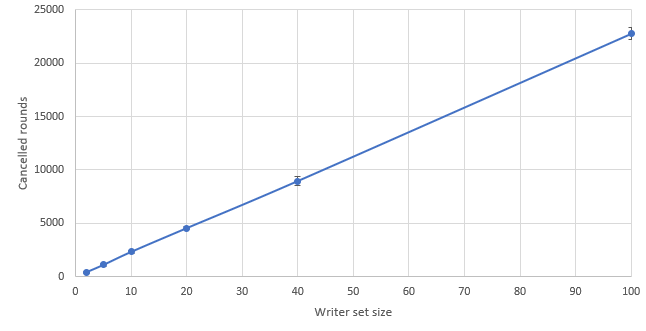
\includegraphics[scale = 0.65]{images/graf.PNG}
    \caption{Growth of the average number of cancelled rounds for different writer set size, mean downtime = 28.800 rounds.}
    \label{fig:failure_rate}
\end{figure}



\section{Applications of the block-chain system +}


%Separate the mechanisms of the block-chain from financial transactions, or the revamping of monetary systems. 

We have experimented with a number of applications enabled by the basic functionality of the light-weight block-chain system. Three of them are briefly discussed below.

\subsection{Digital Certification Service}
A Digital Certification Service in its purest form is essentially a time-stamping service, merely evidencing that the digital object written into the chain existed at a certain time relative to other events on the chain. Adding a (local) timestamp to the body, with the writers participating in the Network Time Protocol \cite{NTP}, provides absolute time of events correct within tens or at most hundreds of milliseconds. For usability, additional information may be collected, written to the body of block, and/or stored in an affiliated database system.

We have implemented a certification service for academic transcripts and diplomas, as a web service. A client submits a document (using the web services API, or manually using a web front end). The service computes a hash of the document and writes it into the block-chain. A reference "ticket" in the form of a QR code is returned to the client. Any third party, having a read access to the chain, can read the chain (using the ticket to speed up its search), compute the document hash and verify when and where it was written in the chain.


\subsection{Traceability service}
We define a traceability service, as the ability to track events related to a named object. We employ a hierarchical naming system, allowing a named object to be broken into parts. In addition some service specific attributes are written to the body. The motivation is to be able to trace objects (and/or their electronic twins) from the source, with applications in food, news, data, and even decisions.

Apart from the naming scheme, the traceability service builds on and uses the digital certification service. An observer verifies the source by selecting all the events matching the name, identifying the first such event in the log.
%The benefits of this service is giving users a secure database for tracing a product through its production, thereby reducing both time and cost of essential inspections done by different entities.
%This service gives users a secure and traceable database for all the steps of the productions, reducing time and cost of various inspections done by different entities.

\subsection{e-Wallets}

We define an e-wallet as a named object having \emph{(attribute,value)} pairs, whose current value is stored in the value and address is stored in the attribute. The application is built upon the traceability service where the e-wallet traces all transactions to and from the wallet's address in the block-chain. A transaction is defined as the wallets owner transferring funds from its e-wallet to another address and cryptographically signing the transaction to prevent spoofing. 

This application can be implemented on the client side or as a web service, storing the data in the cloud. When users register a wallet, they are given a public private key pair, where the public key is the wallets address and the private key is used for signing the transactions. The e-wallet is safe as long as the users private key is secure. 


%\section{Future work}
%Automatically change the membership of the set of writers – possibly using our voting %scheme for that

%\section*{discussion}

%This template automatically loads usual \verb+amsthm+ and \verb+amsmath+ packages.  %Additional packages should be loaded in the preamble.  

\section{conclusions}
In this paper we have proposed a lightweight blockchain protocol. It shows superior scalability over the popular PoW consensus since it requires no hashing and is computationally inexpensive. In a practical setting, where nodes can go offline or need maintenance, a consensus will not be reached. In that case we have introduced a cancellation policy in which that round is deemed unsuccessful and the next round starts. To combat repeated cancellations, nodes will be put in a penalty box with an exponential wait, so that if it goes offline for many hours, it will only cancel tens of rounds. Simulations of this protocol have shown that in a practical setting, consensus is reached in over 99\% of the rounds for at least 97\% of the players, as was shown in Section \ref{simulation-res}. 

This protocol is not attached to any particular application, but it supports such integration. We have demonstrated a few applications that utilizes the advantages of the blockchain for their features. It can also be used as a building block for a new cryptocurrency using e-wallets, which we will be working on in the future.

%\section*{acknowledgements}
%This section is optional. The authors thank and not ``would like to thank'' such and such an organization or person. Co-authors should not be listed here.
%Note correct LaTeX quotations above. Do not use the " symbol, but rather double ` followed by double '


%Use no indents. Follow the style given in the examples (journals and serial publications;\cite{journal} chapters and monographs;\cite{chapters} web sources,\cite{web} correspondingly) below. All references in text must be in order of appearance. Please include all authors, the complete title, and inclusive pagination, \textit{e.g.}, 1234--1237, not 1234--7; \ul{please make sure to use en-dash} (in \LaTeX, use \verb+--+) \ul{and not the regular dash or em-dash to indicate duration between page numbers or years.} The publication year should follow authors in parentheses. Supply DOI numbers whenever possible. \textit{Book titles} and \textit{web sites} are italicized. \textit{Titles of journals} should be abbreviated according to http://www.abbreviations.com/jas.php. \textbf{\ul{Reference accuracy is critical. It is authors responsibility to carefully check each reference.}} 

%In the text, separate superscripted numbers by comma and space,\cite{journal,chapters} they should be separated by an en-dash if the consecutive list of more than two numbers is used.\cite{journal,chapters,web} List them AFTER punctuation (be it comma or period) with no space.

\printbibliography{}

% The About the Student Author section is NOT optional.  Write a paragraph about the student; see previous journal editions for examples.
% If there is more than one student author, you must move the comment below.
%\section*{about the student author}
%\section*{about the student authors}
%John Smith and Jane Smith will graduate in \ldots, \textit{etc.}

% The Press Summary section is NOT optional.  Write a paragraph describing the paper in a manner suitable for the press; see previous journal editions for examples.
%\section*{press summary}

%Please rewrite your abstract so that it captures in few sentences the scope and focus of your publication but could be easily understood by the general public and hopefully shows why your work is exciting and important.



\end{document}
